\section{Evaluation} % 2 pages 
\label{sec:results}
To run our deep RL algorithms we use RLlib~\cite{liang2017rllib}, an open-source library for reinforcement learning that offers both high scalability and a unified API for a variety of applications. RLlib is built on top of Ray~\cite{moritz2018ray}, a high-performance distributed execution framework targeted at large-scale machine learning and reinforcement learning applications. We ran the framework on a four-core Intel i7-4765T CPU%~\cite{Intel2017}
with a Tesla K20c GPU% ~\cite{Nvidia2012}
for training and inference. 

We set our frequency constraint in HLS to 200MHz and use the number of clock cycles reported by the HLS profiler as the circuit performance metric.
In~\cite{huang2013effect}, results showed a one-to-one correspondence between the clock cycle count and the actual hardware execution time under certain frequency constraint. Therefore, better clock cycle count will lead to better hardware performance.
\subsection{Performance}
To evaluate the effectiveness of various algorithms for tackling the phase-ordering problem, we run them on nine real HLS benchmarks and compare the results based on the final HLS circuit performance and the sample efficiency against state-of-the-art approaches for overcoming the phase ordering, which include random search, Greedy Algorithms~\cite{huang2013effect}, OpenTuner~\cite{ansel2014opentuner}, and Genetic Algorithms~\cite{DEAP_JMLR2012}. These benchmarks are adapted from CHStone~\cite{hara2008chstone} and LegUp examples. They are: \emph{adpcm}, \emph{aes}, \emph{blowfish}, \emph{dhrystone}, \emph{gsm}, \emph{matmul}, \emph{mpeg2}, \emph{qsort}, and  \emph{sha}.
For this evaluation, the input features/rewards were not normalized, the pass length was set to 45, and each algorithm was run on a per-program basis. Table~\ref{tab3} lists the action and observation spaces used in all the deep RL algorithms.
\begin{table*}[!t]
\scriptsize
\centering
\caption{The observation and action spaces used in the different deep RL algorithms.}
\label{tab3}
\begin{tabu}{|[1.2pt]c|[1.2pt]c|c| c|c|c|[1.2pt]}
\tabucline[1.2pt]{-}

& \textbf{RL-PPO1} & \textbf{RL-PPO2} & \textbf{RL-PPO3} & \textbf{RL-A3C} & \textbf{RL-ES} \\ \hline
\tabucline[1.2pt]{-}

\textbf{Deep RL Algorithm} & PPO & PPO & PPO & A3C & ES \\ \hline
\textbf{Observation Space} & Program Features & Action History &  Action History + Program Features & Program Features & Program Features \\ \hline
\textbf{Action Space} & Single-Action & Single-Action & Multiple-Action & Single-Action & Single-Action \\ \hline
\tabucline[1.2pt]{-}

\end{tabu}
\end{table*}
 
The bar chart in Figure~\ref{fig:train_result} shows the percentage improvement of the circuit performance compared to -O3 results on the nine real benchmarks from CHStone. The dots on the blue line in Figure~\ref{fig:train_result} show the total number of samples for each program, which is the number of times the algorithm calls the simulator to gather the cycle count.   
%Here is a summary on all the configurations we evaluate. 
\texttt{-O0} and \texttt{-O3} are the default compiler optimization levels. 
\texttt{RL-PPO1} is a PPO explorer where we set all the rewards to 0 to test if the rewards are meaningful. 
\texttt{RL-PPO2} is the PPO agent that learns the next pass based on a histogram of applied passes. 
\texttt{RL-A3C} is the A3C agent that learns based on the program features.
\texttt{Greedy} performs the greedy algorithm, which always inserts the pass that achieves the highest speedup at the best position (out of all possible positions it can be inserted to) in the current sequence. 
\texttt{RL-PPO3} uses a PPO agent and the program features but with the action space described in Section~\ref{subsubsec:conf2}.
explained in Section~\ref{subsubsec:conf2}. 
\texttt{OpenTuner} runs an ensemble of six algorithms, which includes two families of algorithms: particle swarm optimization~\cite{kennedy2010particle} and GA,
each with three different crossover settings. %PSO_GA_Bandit
\texttt{RL-ES} is similar to A3C agent that learns based on the program features, but updates the policy network using the evolution strategy instead of backpropagation.  
\texttt{Genetic-DEAP}~\cite{DEAP_JMLR2012} is a genetic algorithm implementation. 
\texttt{random} randomly generates a sequence of 45 passes at once instead of sampling them one-by-one.  

From \texttt{Greedy}, we see that always adding the pass in the current sequence that achieves the highest reward leads to sub-optimal circuit performance.
\texttt{RL-PPO2} achieves higher performance than \texttt{RL-PPO1}, which shows that the deep RL captures useful information during training. Using the histogram of applied passes results in better sample efficiency, but using the program features with more samples results in a slightly higher speedup.  
\texttt{RL-PPO2}, for example, at the minor cost of 4\% lower speedup, achieves 50$\times$ more sample efficiency than \texttt{OpenTuner}. 
Using ES to update the policy is supposed to be more sample efficient for problems with sparse rewards like ours, however, our experiments did not benefit from that. 
Furthermore, \texttt{RL-PPO3} with multiple action updates achieves a higher speedup than the other deep RL algorithms with a single action. One reason for that is  the ability of \texttt{RL-PPO3} to explore more passes per compilation as it applies multiple passes simultaneously in between every compilation. On the other hand, the other deep RL algorithms apply a single pass at a time. 

%OpenTuner and uses a bandit algorithm to pick the best algorithms to run. Move to background

\begin{figure}[!t]
    \centering
    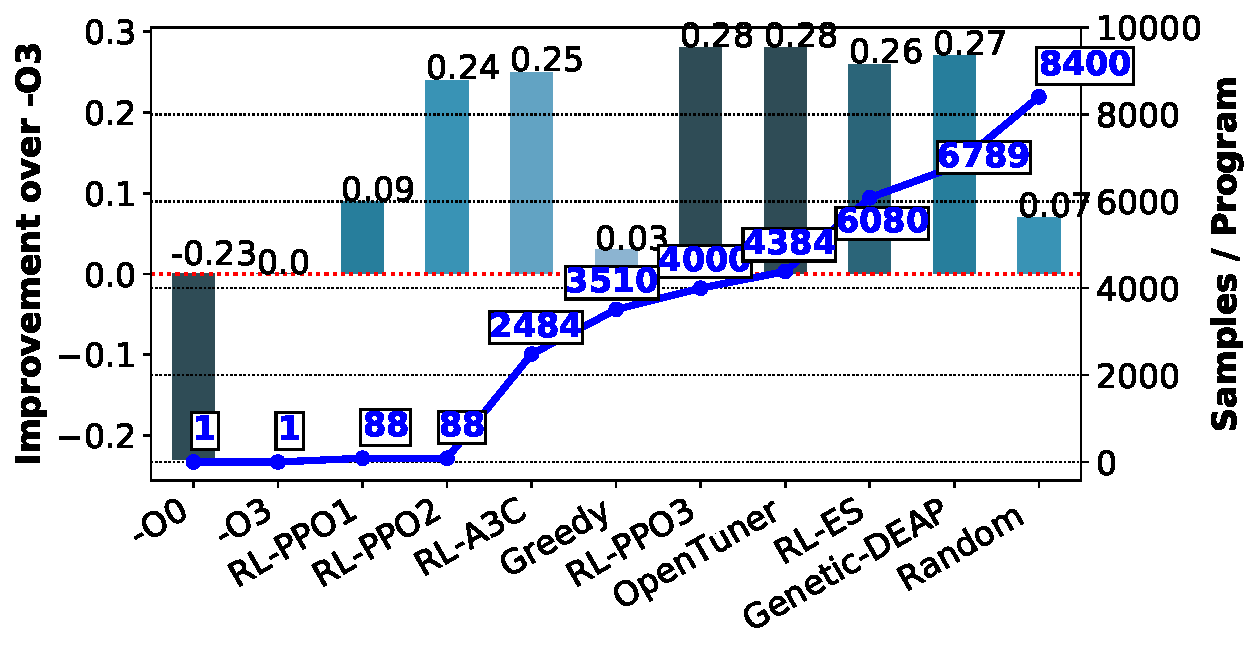
\includegraphics[width=0.5\textwidth]{Figures/train_result.pdf}
    \vspace{-0.5cm}
    \caption{Circuit Speedup and Sample Size Comparison.}
    \label{fig:train_result}
\end{figure}
%\vspace{-20pt}


\subsection{Generalization}
%Training on different programs and benchmarks and then using the trained network to inference on any existing program and expect it to achieve optimal results is not practical. Yet, 

With deep RL, the search should benefit from prior knowledge learned from other different programs. This knowledge should be transferable from one program to another. For example, as discussed in section~\ref{sec:features} applying pass \textit{-loop-rotate} is always beneficial, and \textit{-loop-unroll} should be applied after \textit{-loop-rotate}. Note that the black-box search algorithms, such as OpenTuner, GA, and greedy algorithms, cannot generalize. For these algorithms, rerunning a new search with many compilations is necessary for every new program, as they do not learn any patterns from the programs to direct the search and can be viewed as a smart random search. %Therefore, these algorithms need to perform a completely new search for every program. 

To evaluate how generalizable deep RL could be with different programs and whether any prior knowledge could be useful, we train on 100 randomly-generated programs using PPO. Random programs are used for transfer learning due to lack of sufficient benchmarks and because it is the worst-case scenario, \textit{i.e.}, they are very different from the programs that we use for inference. The improvement can be higher if we train on programs that are similar to the ones we inference on. We train a network with $256\times256$ fully connected layers and use the histogram of previously applied passes concatenated to the program features as the observation and passes as actions. 

%We normalized the program features to the total number of instructions.
As described in Section~\ref{subsection:norm}, we experiment with two normalization techniques for the program features: \textcircled{1} taking the logarithm of all the program features and \textcircled{2} normalizing the program features to the total number of instructions in the program.  
In each pass sequence, the intermediate reward was defined as the logarithm of the improvement in cycle count after applying each pass. The logarithm was chosen so that the RL agent will not give much larger weights to big rewards from programs with longer execution time. Three approaches were evaluated: \texttt{filtered-norm1}
uses the filtered (based on the analysis in Section~\ref{sec:features} where we only keep the important features and passes) program features and passes from Section with normalization technique \textcircled{1}, \texttt{original-norm2} uses all the program features and passes with normalization technique \textcircled{2}, and \texttt{filtered-norm2} uses the filtered program features and passes from Section~\ref{sec:features} with normalization technique \textcircled{2}. 
%data we analyzed from section~\ref{sec:features} where we keep only the impactful features and passes. 
Filtering the features and passes might not be ideal, especially when different programs have different feature characteristics and impactful passes. However, reducing the number of features and passes helps to reduce variance among all programs and significantly narrow the search space. % that will make the learning process easier and faster.

\begin{figure}[!t]
    \centering
    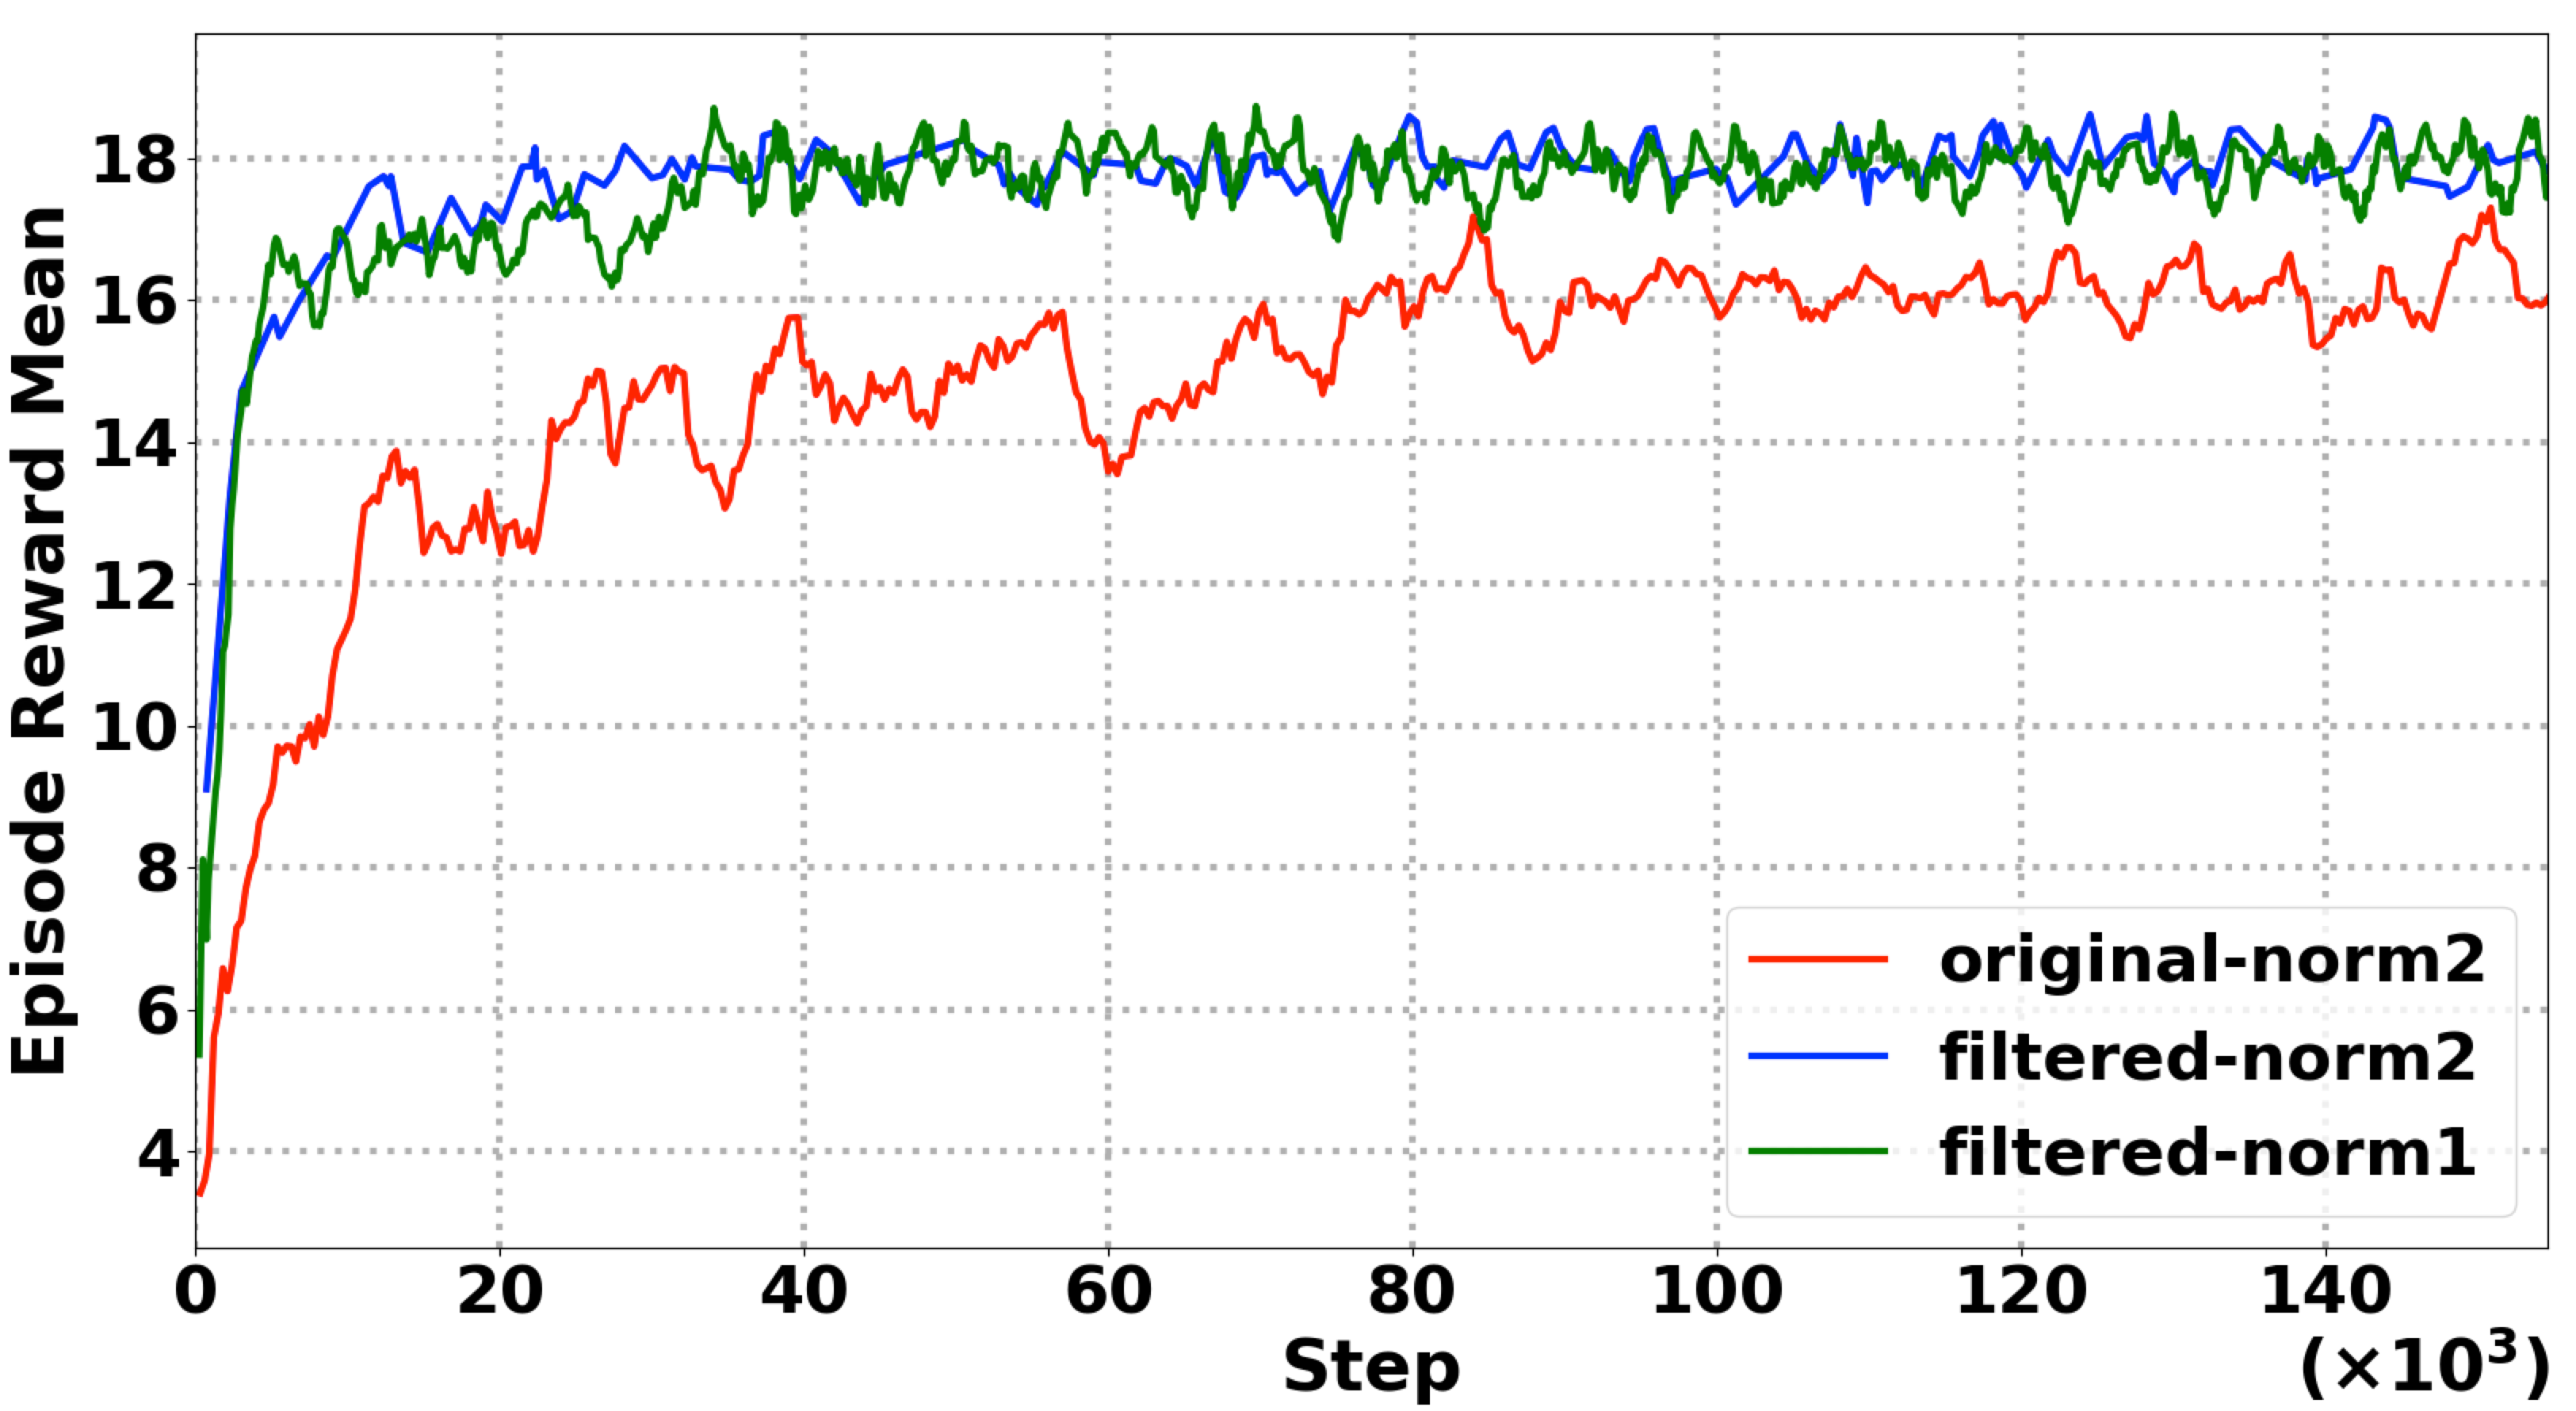
\includegraphics[width=\linewidth]{Figures/reward2.png}
    \caption{Episode reward mean as a function of step for the original approach where we use all the program features and passes and for the filtered approach where we filter the passes and features (with different normalization techniques). Higher values indicate faster circuit speed.}
    \label{fig:reward}
\end{figure}
Figure~\ref{fig:reward} shows the episode reward mean as a function of the step for the three approaches. We observe that \texttt{filtered-norm2} and \texttt{filtered-norm1} converge much faster and achieve a higher episode reward mean than \texttt{original-norm2}, which uses all the features and passes. At roughly 8,000 steps the \texttt{filtered-norm2} and \texttt{filter-norm1} already achieve a very high episode reward mean, with minor improvements in later steps. Furthermore, the episode reward mean of the filtered approaches is still higher than that of \texttt{original-norm2} even when we allowed it to train for 20 times more steps (\textit{i.e.}, 160,000 steps). This indicates that filtering the features and passes significantly improved the learning process. 
All three approaches learned to always apply pass \textit{-loop-rotate}, and \textit{-loop-unroll} after \textit{-loop-rotate}. Another useful pass that the three approaches learned to apply is \textit{-loop-simplify}, which performs several transformations to transform natural loops into a simpler form that enables subsequent analyses and transformations.

%We later use both networks to inference (rollout) the CHStone benchmarks and LegUp examples as well as other 12874 randomly generated programs. Interestingly, the network with all the features and passes delivered 7\% worse results than \mbox{-O3} while the filtered one delivered 6\% better results than -O3 with only 5\% of the programs performing slightly worse (less than 1\%) than -O3. While in general having more passes and features should give better performance, filtering the features and passes helped reduce the variance and enabled better learning of data that could be transferred to other programs more efficiently.
% simpler and more effective. 
%This pass will clean up blocks which are split out, but end up being unnecessary, so usage of this pass should not deteriorate generated code. 

We now compare the generalization results of \texttt{filtered-norm2} and \texttt{filtered-norm1} with the other black-box algorithms. We use 100 randomly-generated programs as the training set and nine real benchmarks from CHStone as the testing set for the deep RL-based methods.
With the state-of-the-art black-box algorithms, we first search for the best pass sequences that achieved the lowest aggregated hardware cycle counts for the 100 random programs and then directly apply them to the nine test set programs.   
In Figure~\ref{fig:train_result_generalization}, the bar chart shows the percentage improvement of the circuit performance compared to -O3 on the nine real benchmarks, the dots on the blue line show the total number of samples each inference takes for one new program.

This evaluation shows that the deep RL-based inference achieves higher speedup than the predetermined sequences produced by the state-of-the-art black-box algorithms for new programs. The predetermined sequences that are overfitted to the random programs can cause poor performance in unseen programs (\textit{e.g.,} -24\% for \texttt{Genetic-DEAP}).  
Besides, normalization technique \textcircled{2} works better compared to normalization technique\textcircled{1} for deep RL generalization (4\% vs 3\% speedup).
This indicates that normalizing the different instructions to the total number of instructions \textit{i.e.}, the distribution of the different instructions in Technique~\textcircled{2} represents more universal characteristics across different programs, 
while taking the log in Technique~\textcircled{1} only suppresses the value ranges of different program features. Furthermore, when we use other 12,874 randomly generated programs as the testing set with \texttt{filtered-norm2}, the speedup is 6\% compared to -O3.
%Lastly, the sample size of the RL methods is higher than one and is equal to the total number of actions to take in each RL trajectory for each inference. We set the trajectory length to 16 in this experiment.

\begin{figure}[!t]
    \centering
    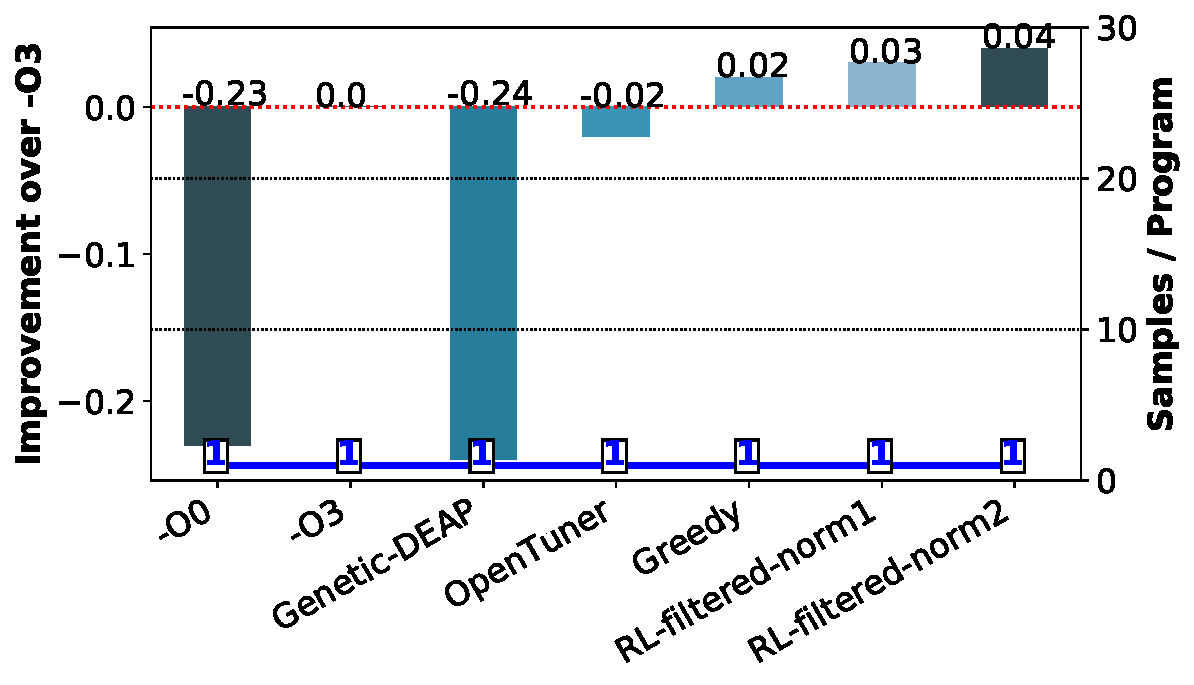
\includegraphics[width=1\linewidth]{Figures/train_result_generalization.pdf}
    \vspace{-0.5cm}
    \caption{Circuit Speedup and Sample Size Comparison for deep RL Generalization.}
    \label{fig:train_result_generalization}
\end{figure} 


